\chapter{Background\label{background}}
Node.js is a asynchronous event-driven JavaScript runtime environment that is designed to build scalable network applications (\cite{node.jsAbout}).
In its core process it uses event loop at runtime to handle callbacks.
Node.js is internally compiled by V8 JavaScript engine using just in time complication (\cite{nodejsTheV8}).

Node.js uses small number of threads to handle many clients rather than using hardware resources for maintaining multiple threads (\cite{node.jsOverviewBlockVsNonBlock}).
Node.js is able to perform blocking I/O event within a single runtime thread by offloading operations to system kernel when possible (\cite{node.jsEventLoop}).
These operations are called non-blocking operations or asynchronous operations (\cite{node.jsOverviewBlockVsNonBlock}).
Events that block the event loop from continuing its process are called blocking operations or synchronous operations.
When thread becomes blocked it can't handle other events until the blocked event is handleded.

Node.js event loop consist of six phases shown in figure \ref{figure:nodejs:eventloop} (\cite{node.jsEventLoop}).
\begin{itemize}
    \item
    timers: executes timers callbacks. Scheduled by \textit{setTimeout} and \textit{setInterval} callbacks.
    \item
    pending callbacks: executes I/O callbacks deferred to the next loop iteration.
    \item
    idle, prepare: only used internally
    \item
    poll: retrieve new I/O events, execute I/O related callbacks.
    \item
    check: \textit{setImmediate} callbacks are invoked here. \textit{setImmediate} executes its callback in the next iteration.
    \item
    close callbacks: emits the 'close' event when socket or handler is closed abruptly
\end{itemize}

\begin{figure}[htbp]
    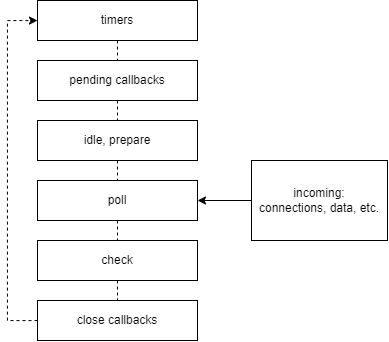
\includegraphics[scale=0.8]{images/event_loop.png}
    \caption{Simplified event loop with it phases. \cite{node.jsEventLoop}.}
    \label{figure:nodejs:eventloop}
\end{figure}

Each phase consist of first in, first out queue of callbacks waiting to be executed.
When event loop enters specific phase it performs callbacks from the queue until the queue is empty or the maximum number of events has been executed.
After that it enters the next phase continuing the process.
Any of these operations may schedule more operations.

Poll phase performs differently when timers or \textit{setImmediate} are called as shown in the figure \ref{figure:nodejs:pollPhase}.
Once the event loop enters the poll phase it executes all callbacks in poll queue synchronously.
After the poll queue is emptied, and there were timers set when the event loop entered poll phase, the event loop will wrap back to timers phase to execute the timers callbacks or keep polling the empty poll queue until timer is exhausted.

When no timers are scheduled when the event loop enters poll phase it executes all callbacks in the poll queue until it is empty or system limit is reached.
When there are scripts called by \textit{setImmediate} and the event loop ends poll phase, it enters the check phase in order to handle the \textit{setImmediate} callbacks.
Otherwise the event loop will wait for callbacks in poll phase and executes callbacks from poll queue immediately.
\begin{figure}[htbp]
    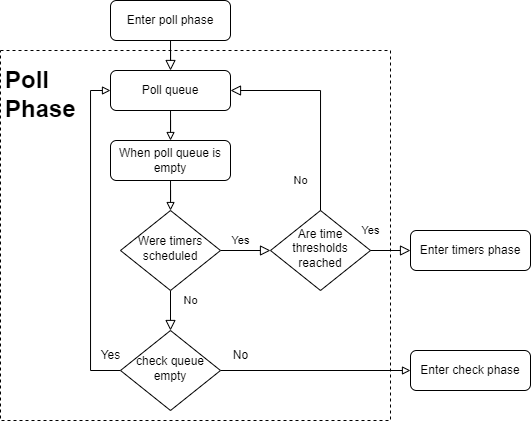
\includegraphics[scale=0.8]{images/poll_phase_flow_chart.png}
    \caption{Poll phase flow chart.}
    \label{figure:nodejs:pollPhase}
\end{figure}